\documentclass[
  12pt,
  headsepline,
  headings=normal,
  toc=bibliography,
  toc=listof
]{scrreport}


%% Variabeln %%%%%%%%%%%%%%%%%%%%%%%%%%%%%%%%%%%%%%%%%%%%%%%%%%%%

\renewcommand{\author}{Guillaume Fournier-Mayer}
\renewcommand{\title}{Rechnergestützter Entwurf digitaler Systeme}

%\RedeclareSectionCommand[tocnumwidth=2.3em]{chapter}
%\RedeclareSectionCommand[tocindent=2.3em,tocnumwidth=3.2em]{section}
\setcounter{secnumdepth}{\subsubsectionnumdepth}
\setcounter{tocdepth}{3}


%% Documentclass Anpassungen
\usepackage{scrhack}


%% Deutsche Anpassungen %%%%%%%%%%%%%%%%%%%%%%%%%%%%%%%%%%%%%
\usepackage[ngerman]{babel}
\usepackage[T1]{fontenc}
\usepackage[utf8]{inputenc}
\usepackage{lmodern} %Type1-Schriftart für nicht-englische Texte
\usepackage{textcomp}


%% Packages für Grafiken & Abbildungen %%%%%%%%%%%%%%%%%%%%%%
\usepackage{graphicx}
%\usepackage{eso-pic}
\usepackage{float}


%% Hyperref %%%%%%%%%%%%%%%%%%%%%%%%%%%%%%%%%%%%%%%%%%%%%%%%%
\usepackage[final, backref=false, pagebackref=false, bookmarks=true]{hyperref}

\hypersetup{ %Ä=\304; Ö=\326; Ü=\334; ä=\344; ö=\366; ü=\374; ß=\377
  pdfauthor={Guillaume Fournier-Mayer},
  pdftitle={EDA-Praktikum},
  pdfsubject={\title},
  pdfproducer={MiKTeX},
  pdfview=FitV,             % Fit, FitH, FitV
  pdfstartview=FitV,        % PDF-Viewer benutzt beim Start bestimmte Seitenbreite
                            % (Fit, FitH, FitV)
  pdfpagemode=UseOutlines,  % PDF-Viewer startet ohne Inhaltsverzeichnis et.al.
                            % (FullScreen, UseOutlines, None)
  linkcolor=black,          % Für Links in der gleichen Seite
  urlcolor=blue,            % Für Links auf URL’s
  breaklinks=false,         % Links dürfen umgebrochen werden
  colorlinks=true,
  citecolor=black,          % Farbe für \cite
  citebordercolor=0 0 0,
  filebordercolor=0 0 0,
  linkbordercolor=0 0 0,
  menubordercolor=0 0 0,
  urlbordercolor=0 0 0,
  pdfhighlight=/I,
  pdfborder=0 0 0,          % keine Box um die Links!
  bookmarksnumbered=false,
  hypertexnames=false,
  bookmarksopen=true
}

%% Geometry %%%%%%%%%%%%%%%%%%%%%%%%%%%%%%%%%%%%%%%%%%%%%%%%%
%\geometry{includeheadfoot, headheight = 17mm, textwidth = 16cm, textheight = 23cm}
\usepackage[left=35mm, right=30mm, top=30mm, bottom=30mm, a4paper]{geometry}

%% TABLE %%%%%%%%%%%%%%%%%%%%%%%%%%%%%%%%%%%%%%%%%%%%%%%%%%%
\usepackage{longtable}
\usepackage{multirow}
%% Header %%%%%%%%%%%%%%%%%%%%%%%%%%%%%%%%%%%%%%%%%%%%%%%%%%%
\usepackage[automark]{scrlayer-scrpage}
\pagestyle{scrheadings}
%\clearpairofpagestyles
\chead{}
\ihead{\headmark}
\automark{chapter}


%% Zitate %%%%%%%%%%%%%%%%%%%%%%%%%%%%%%%%%%%%%%%%%%%%%%%%%%%%%
\usepackage[backend=biber,style=numeric,]{biblatex}
\addbibresource{literatur.bib}
\usepackage{dirtytalk}

%% Formeln %%%%%%%%%%%%%%%%%%%%%%%%%%%%%%%%%%%%%%%%%%%%%%%%%%%%%
\usepackage{amsmath}
\usepackage{nicefrac}

%% Titel %%%%%%%%%%%%%%%%%%%%%%%%%%%%%%%%%%%%%%%%%%%%%%%%%%%%%

%% Dokument %%%%%%%%%%%%%%%%%%%%%%%%%%%%%%%%%%%%%%%%%%%%%%%%%%%%
\begin{document}
%\AddToShipoutPicture{\includegraphics{img/Deckblatt.pdf}}
\begin{titlepage}
  \begin{center}
    
\includegraphics[scale=0.15]{img/wedel_logo.png}\\
    \vspace{1cm}
    \begin{Huge}
      \textbf{\title}\\
    \end{Huge}
    \vspace{1cm}
    \begin{LARGE}
      Kräfteplazierung\\
    \end{LARGE}
    \begin{Large}
      Fachrichtung technische Informatik\\
    \end{Large}
    \vspace{0.5cm}
    \today\\
    Wintersemetester 2021/2022\\
    \vspace{1.5cm}
    \author\\
    tinf-101922\\
    tinf101922@stud.fh-wedel.de\\
  \end{center}
\end{titlepage}
%\ClearShipoutPicture
%\renewcommand{\thechapter}{\Roman{chapter}}
%\pagenumbering{Roman}
\tableofcontents
\newpage
%\renewcommand{\thechapter}{\arabic{chapter}}
%\setcounter{chapter}{0}
%\pagenumbering{arabic}
\chapter{Einleitung}

    \section{Problemstellung}
        Ziel des Praktikums ist es, eine Software zu entwerfen, die einen der Teilschritt Clustering,
        Platzierung oder Verdrahtung im Entwurf digitaler Systeme übernimmt.
        In dieser Arbeit wurde als Teilschritt die Platzierung ausgewählt,
        sodass die übrigen Teilschritte Clustering und Verdrahtung von einer zusätzlichen Software Namens
        \textit{Versatile Place and Route (VPR)} übernommen werden.
        Dabei ist zu erwähnen, dass eine FPGA-Architektur gewählt wird die ein Clustering überflüssig macht.
        Abschließend sollen die Ergebnisse der entworfenen Software mit denen von VPR verglichen werden.
        \\\\
        Der grobe Ablauf des gesamten Entwurfes besteht darin, die Netzliste einzulesen und
        mithilfe der FPGA-Architektur eine passende Platzierung zu ermitteln.
        In der Netzliste, die als *.net Datei abgelegt wird, befinden sich alle Informationen über
        Logikblöcke sowie Eingangs- und Ausgangspins des FPGA und wie diese miteinander verbunden sind.
        Die FPGA-Architektur die als *.arch Datei gespeichert wird beinhaltet Daten über die Beschaffenheit des FPGAs.
        Dazu gehören zum Beispiel Kanalbreite oder der genaue Aufbau der Logikblöcke.
        \\
        War die Platzierung erfolgreich, wird eine Platzierungsdatei *.place mit den Positionen der einzelnen Logikblöcke erstellt.
        Als nächster Schritt ließt VPR die Platzierungsinformationen ein und verdrahtet die Blöcke mithilfe der Netzliste und der FPGA-Architektur.
        Die daraus entstehende *.route Datei beinhaltet wiederum die Informationen wie die Blöcke miteinander verbunden sind.
        Je besser die Platzierung, desto einfacher ist der Verdrahtungsschritt.
        Des Weiteren können schon beim Platzieren verschiedene Optimierungen vorgenommen werden um zum Beispiel den kritischen Pfad zu minimieren.

    \section{Kräfteplatzierung}
        Die Kräfteplatzierung ist ein Platzierungalgorithmus, der in Analogie zu einem System steht, in dem alle Blöcke durch Federn miteinander verbunden sind.
        Dabei üben die Federn in Abhängigkeit zum Abstand der Blöcke Kraft auf diese aus.
        Daraus folgt, dass die optimale Position der einzelnen Blöcke diejenige ist, in der ein Kräftegleichgewicht herrscht.
        Die Kraft (\ref{equ:force}) zwischen zwei Blöcken $a$ und $b$ kann dabei durch das Hooksche Gesetz beschrieben werden, wobei $d_{ab}$ (\ref{equ:euklid}) den euklidischen Abstand zwischen $a$ und $b$
        und $w_ab$ die Gewichtung der Verbindung beschreibt. Für ein Block in einem Netz, der mit $n$ Blöcken verbunden ist,
        ist die Gesamtkraft $F_{ges}$ dementsprechend die Summe aller Kräfte (\ref{equ:force_sum}).

        \begin{align}
            \label{equ:euklid}
            w_{ab} = \sqrt{\Delta{}x_{ab}^2 + \Delta{}y_{ab}^2}\\
            \label{equ:force}
            F = w_{ab} \cdot d_{ab}\\
            \label{equ:force_sum}
            F_{ges} = \sum_{j=1}^{n} (w_{ij} \cdot d_{ij})
        \end{align}

        \subsection{Zero-Force-Target (ZFT)}
            Als Zero-Force-Target wird ein Zustand verstanden, indem ein Block im Kräftegleichgewicht ist.
            Block D befindet sich in der Abbildung (\ref{fig:zft-position}) im Kräftegleichgewicht.
            Seine Position ist somit gleich der ZFT-Position \cite{layout}[S. 107].
            \begin{figure}[H]
                \centering
                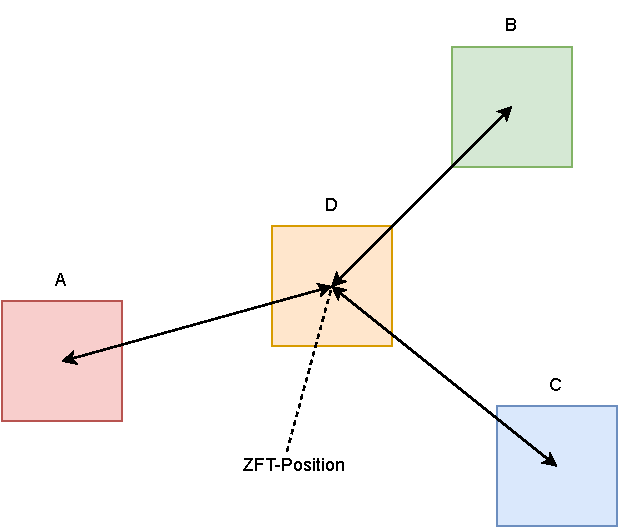
\includegraphics[scale=0.75]{img/zft.pdf}
                \caption{ZFT-Position}
                \label{fig:zft-position}
            \end{figure}
            Zur Bestimmung der ZFT-Position werden die Kräftegleichungen (\ref{equ:Kräftegleichungen})
            null gesetzt und nach der ZFT-Position ($x_i^0$, $y_i^0$) umgestellt sodass
            die Gleichungen (\ref{equ:zft-position}) gebildet werden können \cite{layout}[S. 107].
            \begin{equation}
                \label{equ:Kräftegleichungen}
                \sum_{j} w_{ij} \cdot (x_j^0-x_i^0) = 0~~
                \sum_{j} w_{ij} \cdot (y_j^0-y_i^0) = 0
            \end{equation}
            \begin{equation}
                \label{equ:zft-position}
                x_i^0 = \frac{\sum_{j} w_{ij} \cdot x_j}{\sum_{j} w_{ij}}~~
                y_i^0 = \frac{\sum_{j} w_{ij} \cdot y_j}{\sum_{j} w_{ij}}
            \end{equation}

        \subsection{Grober Ablauf}
            Der grobe Ablauf der Kräfteplatzierung besteht zunächst darin, eine Initialplatzierung zu finden.
            War dies erfolgreich, werden iterativ die ZFT-Position aller Blöcke berechnet.
            Ist die ZFT-Position frei, kann der aktuell betrachtete Block auf die freie Position verschoben werden.
            Ist die Zielposition belegt, muss eine Belegungsoption (\ref{sec:beleungsoptionen}) angewandt werden.
            Ist dies geschehen, wird der nächste Block betrachtet.
            Dies geschieht so lange, bis eine Abbruchbedingung erfüllt ist \cite{layout}[S. 108].

            \begin{enumerate}
                \item Zufällige Initialplatzierung
                \item Berechnen der ZFT-Position des aktuellen Blocks
                        \begin{itemize}
                            \item ZFT-Position ist frei $\rightarrow$ Block auf ZFT-Position verschieben 
                            \item ZFT-Position ist belegt $\rightarrow$ Belegungsoption (\ref{sec:beleungsoptionen}) wählen
                        \end{itemize}
                \item Schritt zwei wiederholen bis Abbruchbedingung erfüllt ist
            \end{enumerate}

        \subsection{Belegungsoptionen}\label{sec:beleungsoptionen}
            \begin{itemize}
                \item Verschieben des Blockes möglichst zu einer Zellenposition nahe der ZFT-Position
                \item Berechnen der Kostenveränderung beim Austausch von zwei Blöcken. Bei verringerten Kosten werden die Blöcke getauscht
                \item \textbf{Chain Move}: Der zu verschiebende Block wird an die Zielposition verschoben,
                    ohne die Kostendifferenz zu berechnen. Der verdränge Block wird auf die nächstgelegende Position verschoben.
                    Ist diese auch belegt, kommt es zu einer Kettenverschiebung (Chain Move)
                \item \textbf{Ripple Move}: Der zu verschiebende Block wird an die Zielposition verschoben und fixiert.
                    Die ZFT-Position des verdrängten Blockes wird berechnet und nach demselben Prinzip verschoben.
                    Dies geschieht so lange, bis alle Blöcke fixiert bzw. platziert sind.
            \end{itemize}\cite{layout}[S. 107f]

            
            





       
        



\chapter{Umsetzung}
\chapter{Auswertung}

%\pagenumbering{Roman}
%\renewcommand{\thechapter}{\Roman{chapter}}
\newpage
\listoffigures
\listoftables
\printbibliography
\end{document}